\documentclass[convert={density=100,outext=.png}]{standalone}
\usepackage{tikz}
\usetikzlibrary{arrows}

\begin{document}
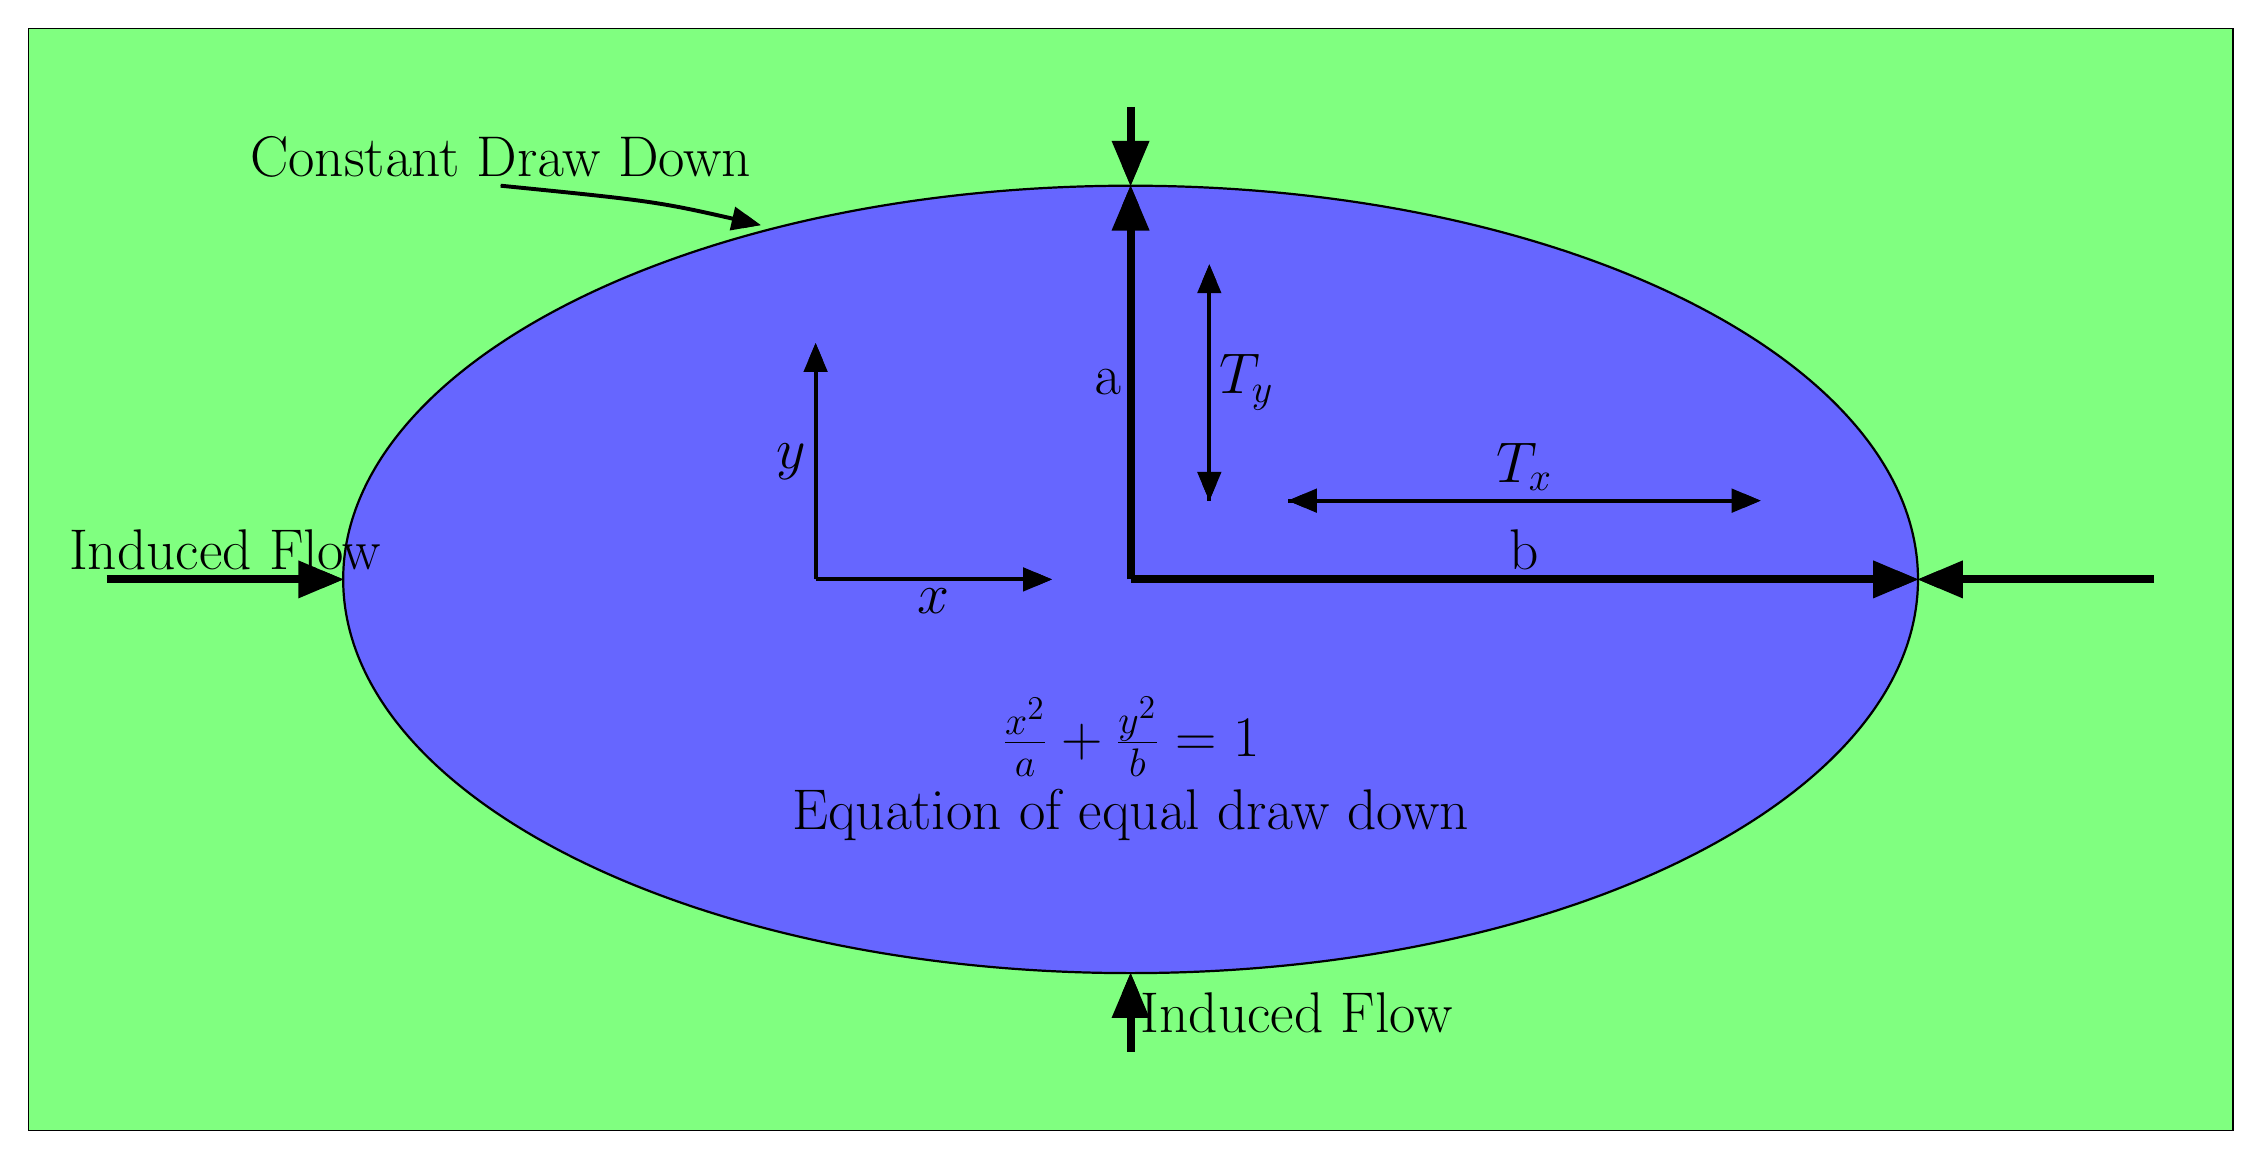
\begin{tikzpicture}
\tikzstyle{normarrow}=[line width=.25mm,-triangle 45,postaction={draw,
  line width=1mm }]
\tikzstyle{arrow}=[line width=.12mm,-triangle 45,postaction={draw,line
  width=.5mm}]
\tikzstyle{every node}=[font=\huge]

\draw[fill=green!50] (-14,-7) rectangle (14,7);
%ellipse size
\draw[fill=blue!60,thick] (0,0) ellipse (10 and 5);

%arrows of a and b
\draw [normarrow] (0,0) -- (0,5) node[pos=.5,left] {a};
\draw[normarrow] (0,0) -- (10,0) node[pos=.5,above] {b};

%arrows of grid and description of problem
\draw (0,-2) node {$\frac{x^2}{a} + \frac{y^2}{b} =1$};
\draw(0,-3) node {Equation of equal draw down};
\draw[arrow] (-4,0) -- (-4,3) node[pos=.5,left] {$y$};
\draw[arrow] (-4,0) -- (-1,0) node[pos=.5,below] {$x$};
\draw[arrow] (1,1) --  (1,4) node[pos=0.5,right] {$T_y$};
\draw[arrow] (1,3) -- (1,1);
\draw[arrow] (2,1) -- (8,1) node[pos=.5,above] {$T_x$};
\draw[arrow] (5,1) -- (2,1);

%induced flow
\draw [normarrow] (0,-6) -- (0,-5) node[pos=.5,right] {Induced Flow};
\draw [normarrow] (0,6) -- (0,5);

\draw[normarrow] (-13,0) -- (-10,0) node [pos=.5, above] {Induced Flow};
\draw[normarrow] (13,0) -- (10,0);

\draw[arrow] (-8,5) .. controls (-6,4.8) .. (-4.7,4.5)
node[pos=0,above] {Constant Draw Down}; 



\end{tikzpicture}
\end{document}